% http://tex.stackexchange.com/questions/109871/two-fills-between-functions-calculated-by-pgfplots?rq=1
\documentclass{standalone}
\usepackage{tikz, pgfplots}
\usetikzlibrary{patterns}
\usepgfplotslibrary{fillbetween}
\begin{document}
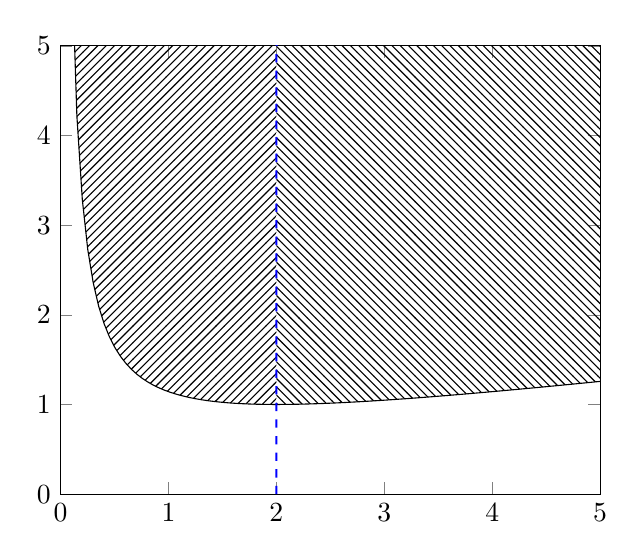
\begin{tikzpicture}
    \begin{axis}[xmin=0,xmax=5,ymin=0,ymax=5]
    \addplot [name path=f,domain=0:5,samples=100] 
        {(x - 2)^2/(7*x) + 1};
		% FIXME : artificial point (5,15) -- would be cool if that
		% could be done automagically
    \addplot [name path=border,color=blue, thick, dashed] plot coordinates {(2,0) (2,5) (5,15)} ;

% FIXME : XOR matching for reverse=true vs false 
	\addplot fill between[of=f and border,reverse=false,split,
		every segment no 0/.style={pattern=north east lines},
		every segment no 1/.style={fill=none},
		soft clip second={(axis cs:1,1) rectangle (axis cs:5,50)},
	];

	\addplot fill between[of=f and border,reverse=true,split,
		every segment no 0/.style={fill=none},
		every segment no 1/.style={pattern=north west lines},
		soft clip second={(axis cs:1,1) rectangle (axis cs:5,50)},
	];
    \end{axis}
\end{tikzpicture}
\end{document}
